\documentclass{beamer}

% \usepackage[lined,ruled]{algorithm2e}
\usepackage{subfigure}
\usepackage[english]{babel}
\usepackage[latin1]{inputenc}
\usepackage{times}
\usepackage[T1]{fontenc} 
\usepackage{color}

\usepackage{listings}
\usepackage{algorithm}
\usepackage{algpseudocode}
\usepackage{paralist}

% "define" Scala
\lstdefinelanguage{scala}{
  morekeywords={abstract,case,catch,class,def,%
    do,else,extends,false,final,finally,%
    for,if,implicit,import,match,mixin,%
    new,null,object,override,package,%
    private,protected,requires,return,sealed,%
    super,this,throw,trait,true,try,%
    type,val,var,while,with,yield, textFile, filter, cache, count,
    flatMap, map, reduceByKey, saveAsTextFile},
  otherkeywords={=>,<-,<\%,<:,>:,\#,@, <+=},
  sensitive=true,
  morecomment=[l]{//},
  morecomment=[n]{/*}{*/},
  morestring=[b]",
  morestring=[b]',
  morestring=[b]"""
}

\usepackage{color}
\definecolor{dkgreen}{rgb}{0,0.6,0}
\definecolor{gray}{rgb}{0.5,0.5,0.5}
\definecolor{mauve}{rgb}{0.58,0,0.82}
 
% Default settings for code listings
\lstset{frame=tb,
  language=scala,
  aboveskip=3mm,
  belowskip=3mm,
  showstringspaces=false,
  columns=flexible,
  basicstyle={\small\ttfamily},
  numbers=left,
  numberstyle=\tiny\color{gray},
  keywordstyle=\color{blue},
  commentstyle=\color{dkgreen},
  stringstyle=\color{mauve},
  frame=single,
  breaklines=true,
  breakatwhitespace=true
  tabsize=3
}


\usetheme[secheader]{Boadilla}
\usefonttheme[onlylarge]{structurebold}
\setbeamerfont*{frametitle}{size=\normalsize,series=\bfseries}
\setbeamertemplate{navigation symbols}{}
\setbeamertemplate{mini frames}[box]
\setbeamertemplate{sections/subsections in toc}[square]
\setbeamertemplate{blocks}[rounded][shadow=true]
\setbeamertemplate{bibliography item}[text]

\setbeamercolor{lightorange}{fg=black,bg=orange!40}
\setbeamercolor{lightblue}{fg=black,bg=blue!30}

\newenvironment{colorblock}[2]
{\setbeamercolor{item}{fg=#1,bg=#1}\begin{beamerboxesrounded}[upper=#1,lower=#2,shadow=true]}
  {\end{beamerboxesrounded}}



% Setup TikZ

\usepackage{tikz}
\usetikzlibrary{arrows}
\tikzstyle{block}=[draw opacity=0.7,line width=1.4cm]


%%%%%%%%%%%%%%%%%%%%%%%%%%%%%%%%%%%%%
%%%%%%%%%%%%%%%%%%%%%%%%%%%%%%%%%%%%%
%%%%%%%%%%%%%%%%%%%%%%%%%%%%%%%%%%%%%

\newtheorem{observation}[theorem]{Observation} 

%%%%%%%%%%%%%%%%%%%%%%%%%%%%%%%%%%%%%
%%%%%%%%%%%%%%%%%%%%%%%%%%%%%%%%%%%%%
%%%%%%%%%%%%%%%%%%%%%%%%%%%%%%%%%%%%%

\title{Introduction to Apache Spark}
% \subtitle{Introduction}
\author{Pietro Michiardi}
\institute{Eurecom}
\date


\begin{document}

\begin{frame}
  \titlepage
\end{frame}

%%%%%%%%%%%%%%%%%%%%%%%%%%%%%%%%%%%%%%%%%%%%%%%%%%%%%%%%%%
\section{Overview}

\begin{frame}
 \begin{colorblock}{blue}{lightblue}{ }
  \begin{center}
    \Huge \textbf{\texttt{Overview}}
  \end{center}
  \end{colorblock}
\end{frame}

\begin{frame}\frametitle{Objectives of the Course}
\begin{itemize}
	\item {\bf Gain hands-on experience on real-life Data Science projects}
	\item {\bf Use knowledge from ``theory'' courses and put them into practice}
	\item {\bf Use knowledge from ``systems'' courses} 
	\item {\bf Develop a methodology to address challenges such as:}
	\begin{itemize}
		\item Data preparation
		\item Data exploration
		\item Algorithm / model selection
		\item Experimental validation and evaluation
	\end{itemize}
\end{itemize}
\end{frame}

\begin{frame}\frametitle{Notebooks, not Lectures!}
\begin{itemize}
	\item {\bf Essentially, there will be no traditional lectures}
	\begin{itemize}
		\item Introduction to machine learning and advanced statistical inference
		\item Distributed systems and cloud computing
		\item Basic computer science skills are necessary
	\end{itemize}

	\item {\bf Notebooks}
	\begin{itemize}
		\item A self-contained studying and development environment
		\item Contains text, reference material, code, questions, graphs
		\item Each Data Science project will be your own project!
	\end{itemize}

	\item {\bf Publish your Notebooks!}
	\begin{itemize}
		\item Create a GitHub account and push your Notebooks there
		\item High-visibility of your own Data Science projects
		\item This is a sort of on-line CV
	\end{itemize}
\end{itemize}
\end{frame}

\begin{frame}\frametitle{Notebooks Content -- Schedule (1)}
\begin{itemize}
	\item {\bf Lab 1 [3/8/2017]}
	\begin{itemize}
		\item Introductory laboratory: getting familiar with Notebooks, Python, Numpy, Pandas, PySpark, Data Frames and more
	\end{itemize}

	\item {\bf Lab 2/3 [3/15/2017 - 3/22/2017]}
	\begin{itemize}
		\item Recommender Algorithms Project: work with real data from an Internet music streaming service, and recommend new music to users
	\end{itemize}

	\item {\bf Lab 4/5 [3/29/2017 - 4/5/2017]}
	\begin{itemize}
		\item Regression Algorithm Project: using random forests to predict airplane delays, using real data from the U.S. DoT
	\end{itemize}
\end{itemize}
\end{frame}

\begin{frame}\frametitle{Notebooks Content -- Schedule (2)}
\begin{itemize}
	\item {\bf Lab 5/6 [4/12/2017 - 4/26/2017]}
	\begin{itemize}
		\item Estimating Financial Risk through Monte Carlo Simulation
	\end{itemize}
	\item {\bf Lab 8/9 [5/3/2017 - 5/10/2017]}
	\begin{itemize}
		\item Clustering Algorithms Project: Anomaly Detection in Network Traffic with $k$-means Clustering
	\end{itemize}
	\item {\bf Industrial Lab [5/24/2017 - 5/31/2017]}
	\begin{itemize}
		\item Industrial Project from SAFRAN Analytics
	\end{itemize}
	\item {\bf Lab 10/11 [6/7/2017]}
	\begin{itemize}
		\item Analyzing Neuro-imaging Data with Thunder
	\end{itemize}
\end{itemize}
\end{frame}


\begin{frame}\frametitle{Industrial Notebooks}
\begin{itemize}
	\item {\bf Great opportunity to be exposed to real industrial problems}
	\begin{itemize}
		\item People from industry supervise the laboratory
		\item Main goal: hiring!
	\end{itemize}
	\item {\bf SAFRAN Analytics}
	\begin{itemize}
		\item \url{http://www.safran-group.com/}
		\item Distribute goodies
		\item Select best student(s) to participate to a SAFRAN event
	\end{itemize}
\end{itemize}
\end{frame}

\begin{frame}\frametitle{How to Be a Successful Student (1)}
\begin{itemize}
	\item {\bf Do not underestimate this course!}
	\begin{itemize}
		\item Be independent and dare to explore and expand your Notebooks
		\item Study or revise the theory: students are assumed to be comfortable with machine learning material, and to follow advanced statistical inference courses
		\item Follow links on the Notebooks. They contain reference material and research papers that: \emph{i)} provide the necessary background; \emph{ii)} offer starting point to improve algorithms
	\end{itemize}
	\item {\bf Is this a course about algorithm design?}
	\begin{itemize}
		\item Sort of: in many cases, Notebooks rely on standard libraries that offer a variety of machine learning algorithms implemented in an efficient way.
		\item Notebooks will illustrate the main algorithmic concepts behind a selection of tools available in such libraries
		\item Advanced (and optional) approaches to those proposed in the Notebooks are more than welcome!
	\end{itemize}
\end{itemize}
\end{frame}

\begin{frame}\frametitle{How to Be a Successful Student (2)}
\begin{itemize}
	\item {\bf Does this course make me a Data Scientist?}
	\begin{itemize}
		\item Sort of: it is the whole track that provides student with the necessary knowledge to start a Data Science career. This course aims at ``learning the hard way'' and put into practice theoretical concepts
	\end{itemize}
	\item {\bf Do I need to know how to program?}
	\begin{itemize}
		\item Yes, and this is mandatory
		\item We will focus on Python, but knowledge of additional languages is definitely a plus
	\end{itemize}
\end{itemize}
\end{frame}

\begin{frame}\frametitle{Grading}
\begin{itemize}
	\item {\bf Grading the laboratories / projects}
	\begin{itemize}
		\item Two-person groups are considered the norm
		\item Each Notebook/project is evaluated and graded
		\item Grading metrics
		\begin{itemize}
			\item Answer to Notebooks questions: this allows you to arrive at 10/20
			\item Depth of answers
			\item Originality of answers and approaches
			\item Additional points to innovative material in each Notebook
		\end{itemize}
	\end{itemize}
	\item {\bf Final exam}
	\begin{itemize}
		\item Depends on class behavior and performance
		\item Example: given a real world Data Science problem, outline an approach to address it, including:
		\begin{itemize}
			\item Relevant data exploration questions
			\item Relevant data cleaning warnings
			\item Model and algorithm selection
			\item Performance considerations
			\item Model validation
		\end{itemize}
	\end{itemize}
\end{itemize}
\end{frame}

\begin{frame}\frametitle{Useful References}
\begin{itemize}
	\item \emph{``An Introduction to Statistical Learning''}, by Gareth James, Daniela Witten, Trevor Hastie and Robert Tibshirani
	\item[] Available for download: \url{http://www-bcf.usc.edu/\~gareth/ISL/}

	\item \emph{``Advanced Analytics with Spark''}, by Sandy Ryza, Uri Laserson, Sean Owen, Josh Wills
	\item[] Available here: \url{http://shop.oreilly.com/product/0636920035091.do}, also available in the Library

	\item \emph{``Understanding Machine Learning: From Theory to Algorithms''}, by Shai Shalev-Shwartz and Shai Ben-David
	\item[] Available for download: \url{http://www.cs.huji.ac.il/~shais/UnderstandingMachineLearning/}
\end{itemize}
\end{frame}

%%%%%%%%%%%%%%%%%%%%%%%%%%%%%%%%%%%%%%%%%%%%%%%%%%%%%%%%%%

%%%%%%%%%%%%%%%%%%%%%%%%%%%%%%%%%%%%%%%%%%%%%%%%%%%%%%%%%%
\section{Anatomy of a Spark Application}

\begin{frame}
 \begin{colorblock}{blue}{lightblue}{ }
  \begin{center}
    \Huge \textbf{\texttt{Anatomy of a Spark Application}}
  \end{center}
  \end{colorblock}
\end{frame}

%%%%%%%%%%%%%%%%%%%%%%%%%%%%%%%%%%%%%%%%%%%%%%%%%%%%%%%%%%
\begin{frame}
\frametitle{Spark Applications: The Big Picture}
%%%%%%%%%%%%%%%%%%%%%%%%%%%%%%%%%%%%%%%%%%%%%%%%%%%%%%%%%%
\begin{itemize}
	\item There are two ways to manipulate data in Spark
	\begin{itemize}
		\item Use the interactive shell, \textit{i.e.,} the REPL
		\item Write standalone applications, \textit{i.e.,} driver programs
	\end{itemize}
\end{itemize}

	\begin{figure}[h]
	  \centering
	  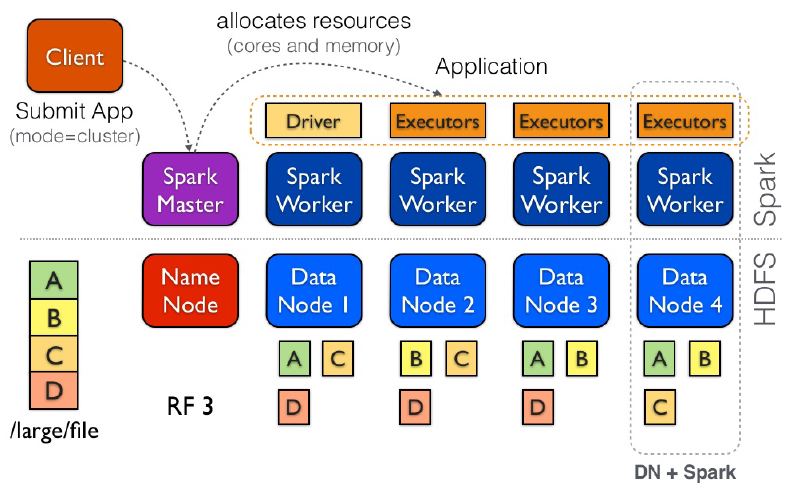
\includegraphics[scale=0.33]{./Figures/spark_app_overview}
	  \label{fig:spark_app_overview}
	\end{figure}
\end{frame}

%%%%%%%%%%%%%%%%%%%%%%%%%%%%%%%%%%%%%%%%%%%%%%%%%%%%%%%%%%
\frame {\frametitle{Spark Components: details}
%%%%%%%%%%%%%%%%%%%%%%%%%%%%%%%%%%%%%%%%%%%%%%%%%%%%%%%%%%
\begin{figure}[h]
  \centering
  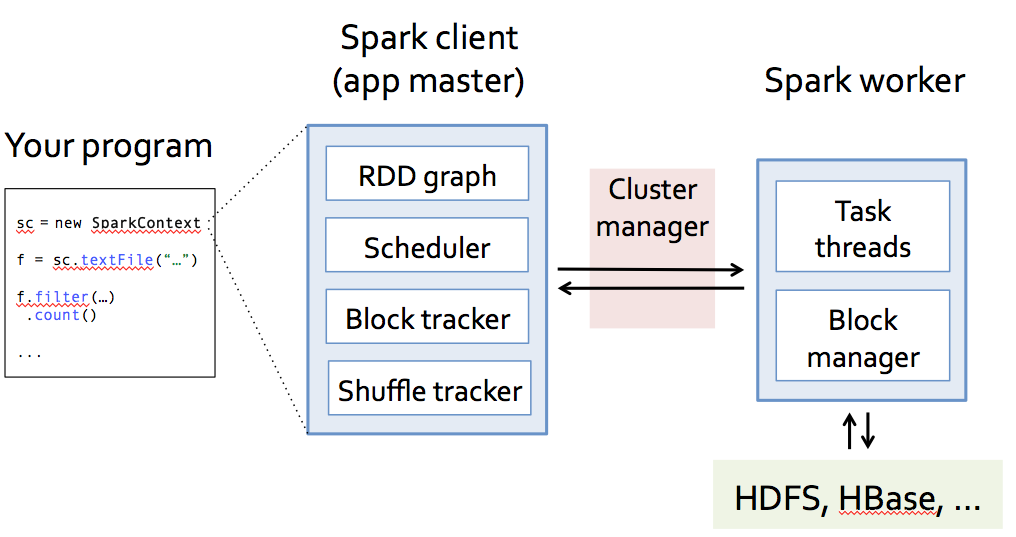
\includegraphics[scale=0.33]{./Figures/spark_components}
  \label{fig:spark_components_details}
\end{figure}
}

%%%%%%%%%%%%%%%%%%%%%%%%%%%%%%%%%%%%%%%%%%%%%%%%%%%%%%%%%%

% %%%%%%%%%%%%%%%%%%%%%%%%%%%%%%%%%%%%%%%%%%%%%%%%%%%%%%%%%%
\frame {\frametitle{In Summary}
% %%%%%%%%%%%%%%%%%%%%%%%%%%%%%%%%%%%%%%%%%%%%%%%%%%%%%%%%%%
\begin{itemize}
	\item {\bf Our example Application}: a \textbf{jar} file
	\begin{itemize}
		\item Creates a \texttt{SparkContext}, which is the core component of the driver
		\item Creates an input RDD, from a file in HDFS
		\item Manipulates the input RDD by applying a \texttt{filter(f: T => Boolean)} transformation
		\item Invokes the action \texttt{count()} on the transformed RDD
	\end{itemize}

	\item {\bf The DAG Scheduler}
	\begin{itemize}
		\item Gets: RDDs, functions to run on each partition and a listener for results
		\item Builds \emph{Stages} of \emph{Tasks} objects (code + preferred location)
		\item Submits Tasks to the \textbf{Task Scheduler} as ready
		\item Resubmits failed \emph{Stages}
	\end{itemize}

	\item {\bf The Task Scheduler}
	\begin{itemize}
		\item Launches \emph{Tasks} on executors
		\item Relaunches failed \emph{Tasks}
		\item Reports to the DAG Scheduler
	\end{itemize}

\end{itemize}

}

%%%%%%%%%%%%%%%%%%%%%%%%%%%%%%%%%%%%%%%%%%%%%%%%%%%%%%%%%%

%%%%%%%%%%%%%%%%%%%%%%%%%%%%%%%%%%%%%%%%%%%%%%%%%%%%%%%%%%
\section{Resilient Distributed Datasets}

\begin{frame}
 \begin{colorblock}{blue}{lightblue}{ }
  \begin{center}
    \Huge \textbf{\texttt{Resilient Distributed Datasets}}
  \end{center}
  \end{colorblock}

  \vspace{20pt}

  \begin{colorblock}{blue}{lightblue}{}
  {\bf M. Zaharia}, M. Chowdhury, T. Das, A. Dave, J. Ma, M. McCauley, M.J. Franklin, S. Shenker, I. Stoica.\\
  \emph{Resilient Distributed Datasets: A Fault-Tolerant Abstraction for In-Memory Cluster Computing},\\
  {\bf USENIX Symposium on Networked Systems Design and Implementation}, 2012    
  \end{colorblock}      


\end{frame}

%%%%%%%%%%%%%%%%%%%%%%%%%%%%%%%%%%%%%%%%%%%%%%%%%%%%%%%%%%
\frame {\frametitle{What is an RDD}
%%%%%%%%%%%%%%%%%%%%%%%%%%%%%%%%%%%%%%%%%%%%%%%%%%%%%%%%%%
\begin{itemize}
	\item {\bf RDD are partitioned, locality aware, distributed collections}
	\begin{itemize}
		\item RDD are \emph{immutable}
	\end{itemize}

	\vspace{20pt}

	\item {\bf RDD are data structures that:}
	\begin{itemize}
		\item Either point to a direct data source (e.g. HDFS)
		\item Apply some transformations to its parent RDD(s) to generate new data elements
	\end{itemize}

	\vspace{20pt}

	\item {\bf Computations on RDDs}
	\begin{itemize}
	 	\item Represented by \emph{lazily evaluated} lineage \emph{DAGs} composed by chained RDDs
	 \end{itemize} 
\end{itemize}
}

%%%%%%%%%%%%%%%%%%%%%%%%%%%%%%%%%%%%%%%%%%%%%%%%%%%%%%%%%%
\frame {\frametitle{RDD Abstraction}
%%%%%%%%%%%%%%%%%%%%%%%%%%%%%%%%%%%%%%%%%%%%%%%%%%%%%%%%%%
\begin{itemize}
	\item {\bf Overall objective}
	\begin{itemize}
		\item Support a wide array of operators (more than just \texttt{Map} and \texttt{Reduce})
		\item Allow arbitrary composition of such operators
	\end{itemize}

	\vspace{20pt}

	\item {\bf Simplify scheduling}
	\begin{itemize}
		\item Avoid to modify the scheduler for each operator
	\end{itemize}

	\vspace{20pt}

	\item[$\to$] The question is: \emph{How to capture dependencies in a general way?}
\end{itemize}
}

%%%%%%%%%%%%%%%%%%%%%%%%%%%%%%%%%%%%%%%%%%%%%%%%%%%%%%%%%%
\frame {\frametitle{RDD Interfaces}
%%%%%%%%%%%%%%%%%%%%%%%%%%%%%%%%%%%%%%%%%%%%%%%%%%%%%%%%%%
\begin{itemize}
	\item {\bf Set of partitions (``splits'')}
	\begin{itemize}
		\item Much like in Hadoop MapReduce, each RDD is associated to (input) partitions
	\end{itemize}

	\item {\bf List of dependencies on parent RDDs}
	\begin{itemize}
		\item This is completely new w.r.t. Hadoop MapReduce
	\end{itemize}

	\item {\bf Function to compute a partition given parents}
	\begin{itemize}
		\item This is actually the ``user-defined code'' we referred to when discussing about the \texttt{Mapper} and \texttt{Reducer} classes in Hadoop
	\end{itemize}

	\item {\bf Optional preferred locations}
	\begin{itemize}
		\item This is to enforce data locality
	\end{itemize}

	\item {\bf Optional partitioning info (Partitioner)}
	\begin{itemize}
		\item This really helps in some ``advanced'' scenarios in which you want to pay attention to the behavior of the shuffle mechanism
	\end{itemize}
\end{itemize}
}

%%%%%%%%%%%%%%%%%%%%%%%%%%%%%%%%%%%%%%%%%%%%%%%%%%%%%%%%%%
\frame {\frametitle{Hadoop RDD}
%%%%%%%%%%%%%%%%%%%%%%%%%%%%%%%%%%%%%%%%%%%%%%%%%%%%%%%%%%
\begin{itemize}
	\item {\color{mauve} partitions} = one per HDFS block

	\vspace{10pt}

	\item {\color{mauve} dependencies} = none

	\vspace{10pt}

	\item {\color{mauve} compute(partition)} = read corresponding block

	\vspace{10pt}

	\item {\color{mauve} preferredLocations(part)} = HDFS block location

	\vspace{10pt}

	\item {\color{mauve} partitioner} = none

\end{itemize}
}

%%%%%%%%%%%%%%%%%%%%%%%%%%%%%%%%%%%%%%%%%%%%%%%%%%%%%%%%%%
\frame {\frametitle{Filtered RDD}
%%%%%%%%%%%%%%%%%%%%%%%%%%%%%%%%%%%%%%%%%%%%%%%%%%%%%%%%%%
\begin{itemize}
	\item {\color{mauve} partitions} = same as parent RDD

	\vspace{10pt}

	\item {\color{mauve} dependencies} = \emph{one-to-one} on parent

	\vspace{10pt}

	\item {\color{mauve} compute(partition)} = compute parent and filter it

	\vspace{10pt}

	\item {\color{mauve} preferredLocations(part)} = none (\emph{ask parent})

	\vspace{10pt}

	\item {\color{mauve} partitioner} = none

\end{itemize}
}

%%%%%%%%%%%%%%%%%%%%%%%%%%%%%%%%%%%%%%%%%%%%%%%%%%%%%%%%%%
\frame {\frametitle{Joined RDD}
%%%%%%%%%%%%%%%%%%%%%%%%%%%%%%%%%%%%%%%%%%%%%%%%%%%%%%%%%%
\begin{itemize}
	\item {\color{mauve} partitions} = one per reduce task

	\vspace{10pt}

	\item {\color{mauve} dependencies} = \emph{shuffle} on \emph{each} parent

	\vspace{10pt}

	\item {\color{mauve} compute(partition)} = read and join shuffled data

	\vspace{10pt}

	\item {\color{mauve} preferredLocations(part)} = none 

	\vspace{10pt}

	\item {\color{mauve} partitioner} = HashPartitioner(numTask)\footnote{Spark knows this data is hashed.}

\end{itemize}
}

%%%%%%%%%%%%%%%%%%%%%%%%%%%%%%%%%%%%%%%%%%%%%%%%%%%%%%%%%%
\frame {\frametitle{Dependency Types (1)}
%%%%%%%%%%%%%%%%%%%%%%%%%%%%%%%%%%%%%%%%%%%%%%%%%%%%%%%%%%
\begin{columns}[t, onlytextwidth]
	\begin{column}[T]{.4\textwidth}
		\begin{center}
			{ \tiny \bf Narrow dependencies}
		\end{center}
		\begin{figure}[h]
			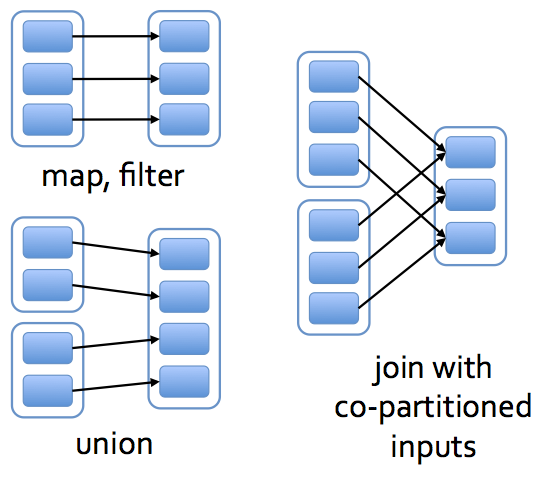
\includegraphics[scale=0.3]{./Figures/narrow_deps}
		\end{figure}
	\end{column}

	\begin{column}[T]{.4\textwidth}
		\begin{center}
			{ \tiny \bf Wide dependencies}
		\end{center}
		\begin{figure}[h]
			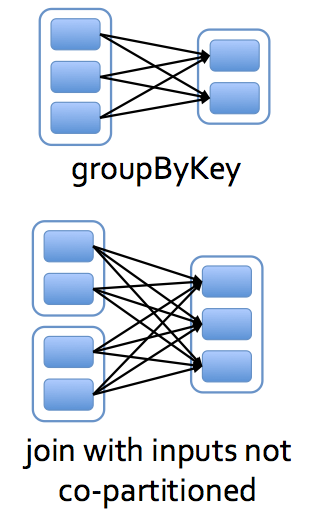
\includegraphics[scale=0.3]{./Figures/wide_deps}
		\end{figure}
	\end{column}
\end{columns}
}

%%%%%%%%%%%%%%%%%%%%%%%%%%%%%%%%%%%%%%%%%%%%%%%%%%%%%%%%%%
\frame {\frametitle{Dependency Types (2)}
%%%%%%%%%%%%%%%%%%%%%%%%%%%%%%%%%%%%%%%%%%%%%%%%%%%%%%%%%%
\begin{itemize}
	\item {\bf Narrow dependencies}
	\begin{itemize}
		\item Each partition of the parent RDD is used by at most one partition of the child RDD
		\item Task can be executed locally and we don't have to shuffle. (Eg: \texttt{map}, \texttt{flatMap}, \texttt{filter}, \texttt{sample})
	\end{itemize}

	\vspace{20pt}

	\item {\bf Wide Dependencies}
	\begin{itemize}
		\item Multiple child partitions may depend on one partition of the parent RDD 
		\item This means we have to shuffle data \textbf{unless the parents are hash-partitioned} (Eg: \texttt{sortByKey}, \texttt{reduceByKey}, \texttt{groupByKey}, \texttt{cogroupByKey}, \texttt{join}, \texttt{cartesian})
	\end{itemize}
\end{itemize}
}

%%%%%%%%%%%%%%%%%%%%%%%%%%%%%%%%%%%%%%%%%%%%%%%%%%%%%%%%%%
\frame {\frametitle{Dependency Types: Optimizations}
%%%%%%%%%%%%%%%%%%%%%%%%%%%%%%%%%%%%%%%%%%%%%%%%%%%%%%%%%%
\begin{itemize}
	\item {\bf Benefits of Lazy evaluation:} The DAG Scheduler optimizes \emph{Stages} and \emph{Tasks} before submitting them to the Task Scheduler
	\begin{itemize}
		\item Examples:
		\begin{itemize}
			\item \textbf{Piplining} narrow dependencies within a Stage
			\item \textbf{Join plan selection} based on partitioning
			\item \textbf{Cache reuse}
		\end{itemize}
	\end{itemize}
\end{itemize}

\begin{figure}[h]
	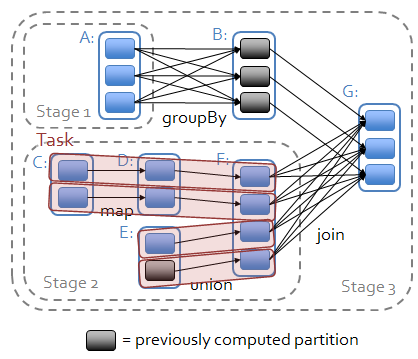
\includegraphics[scale=0.5]{./Figures/deps_optimization}
\end{figure}

}


%%%%%%%%%%%%%%%%%%%%%%%%%%%%%%%%%%%%%%%%%%%%%%%%%%%%%%%%%%
\frame {\frametitle{Operations on RDDs: Transformations}
%%%%%%%%%%%%%%%%%%%%%%%%%%%%%%%%%%%%%%%%%%%%%%%%%%%%%%%%%%
\begin{itemize}
	\item {\bf Transformations}
	\begin{itemize}
		\item Set of operations on a RDD that define how they should be transformed
		\item As in relational algebra, the application of a transformation to an RDD yields a new RDD (because RDDs are \emph{immutable})
		\item Transformations are lazily evaluated, which allow for optimizations to take place before execution
	\end{itemize}

	\vspace{10pt}

	\item {\bf Examples} (not exhaustive)
	\begin{itemize}
		\item \texttt{map(func)}, \texttt{flatMap(func)}, \texttt{filter(func)}
		\item \texttt{grouByKey()}
		\item \texttt{reduceByKey(func)}, \texttt{mapValues(func)}, \texttt{distinct()}, \texttt{sortByKey(func)}
		\item \texttt{join(other)}, \texttt{union(other)}
		\item \texttt{sample()}
	\end{itemize}

\end{itemize}

}

%%%%%%%%%%%%%%%%%%%%%%%%%%%%%%%%%%%%%%%%%%%%%%%%%%%%%%%%%%
\frame {\frametitle{Operations on RDDs: Actions}
%%%%%%%%%%%%%%%%%%%%%%%%%%%%%%%%%%%%%%%%%%%%%%%%%%%%%%%%%%
\begin{itemize}
	\item {\bf Actions}
	\begin{itemize}
		\item Apply transformation chains on RDDs, eventually performing some additional operations (e.g., counting)
		\item Some actions only store data to an external data source (e.g. HDFS), others fetch data from the RDD (and its transformation chain) upon which the action is applied, and convey it to the driver
	\end{itemize}

	\vspace{20pt}

	\item {\bf Examples} (not exhaustive)
	\begin{itemize}
		\item \texttt{reduce(func)}
		\item \texttt{collect()}, \texttt{first()}, \texttt{take()}, \texttt{foreach(func)}
		\item \texttt{count()}, \texttt{countByKey()}
		\item \texttt{saveAsTextFile()}
	\end{itemize}

\end{itemize}
}

%%%%%%%%%%%%%%%%%%%%%%%%%%%%%%%%%%%%%%%%%%%%%%%%%%%%%%%%%%
\frame {\frametitle{Operations on RDDs: Final Notes}
%%%%%%%%%%%%%%%%%%%%%%%%%%%%%%%%%%%%%%%%%%%%%%%%%%%%%%%%%%
\begin{itemize}

	\item {\bf Look at return types!}
	\begin{itemize}
		\item Return type: RDD $\to$ transformation
		\item Return type: built-in scala/java types such as \texttt{int}, \texttt{long}, \texttt{List<Object>}, \texttt{Array<Object>} $\to$ action
	\end{itemize}

	\vspace{10pt}

	\item {\bf Caching is a transformation}
	\begin{itemize}
		\item Hints to keep RDD in memory after its first evaluation
	\end{itemize}

	\vspace{10pt}

	\item {\bf Transformations depend on RDD ``flavor''}
	\begin{itemize}
		\item \texttt{PairRDD}
		\item \texttt{SchemaRDD}
	\end{itemize}

\end{itemize}
}

%%%%%%%%%%%%%%%%%%%%%%%%%%%%%%%%%%%%%%%%%%%%%%%%%%%%%%%%%%
\frame {\frametitle{Common Transformations}
%%%%%%%%%%%%%%%%%%%%%%%%%%%%%%%%%%%%%%%%%%%%%%%%%%%%%%%%%%
\begin{columns}[t, onlytextwidth]
	\begin{column}[T]{.3\textwidth}
		\begin{center}
			\texttt{map(f: T => U)}	
		\end{center}
	\end{column}

	\begin{column}[T]{.5\textwidth}
		
			Returns a \texttt{MappedRDD[U]} by applying $f$ to each element
		
	\end{column}
\end{columns}

\begin{figure}[h]
	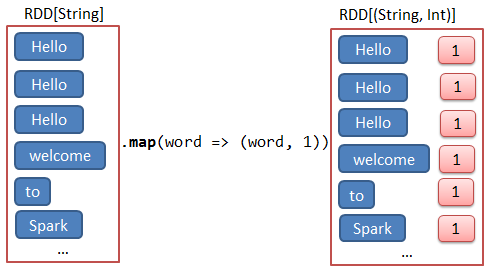
\includegraphics[scale=0.6]{./Figures/transformation_map}
\end{figure}

}

%%%%%%%%%%%%%%%%%%%%%%%%%%%%%%%%%%%%%%%%%%%%%%%%%%%%%%%%%%
\frame {\frametitle{Common Transformations}
%%%%%%%%%%%%%%%%%%%%%%%%%%%%%%%%%%%%%%%%%%%%%%%%%%%%%%%%%%
\begin{columns}[t, onlytextwidth]
	\begin{column}[T]{.4\textwidth}
		\begin{center}
			\texttt{flatMap(f: T => TraversableOnce[U])}	
		\end{center}
	\end{column}

	\begin{column}[T]{.4\textwidth}
		
			Returns a \texttt{FlatMappedRDD[U]} by first applying $f$ to each element, then flattening the results
		
	\end{column}
\end{columns}

\begin{figure}[h]
	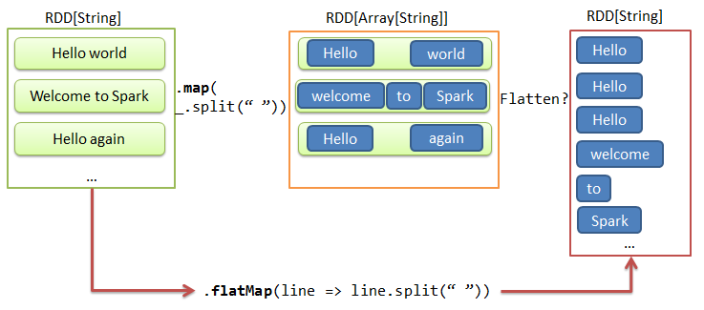
\includegraphics[scale=0.6]{./Figures/transformation_flatmap}
\end{figure}

}



%%%%%%%%%%%%%%%%%%%%%%%%%%%%%%%%%%%%%%%%%%%%%%%%%%%%%%%%%%
\begin{frame}
 \begin{colorblock}{blue}{lightblue}{ }
  \begin{center}
    \Huge \textbf{\texttt{Advanced Topics}}
  \end{center}
  \end{colorblock}
\end{frame}

% \begin{frame}\frametitle{TODO}
% \begin{itemize}
%   \item Data partitioning
%   \item Broadcast Variables
%   \item Accumulators
%   \item MLLib
% \end{itemize}


\begin{frame}\frametitle{Accumulators (1)}
\begin{itemize}
	\item {\bf Underlying idea}
	\begin{itemize}
		\item Simple mechanism and syntax for aggregating values from worker nodes back to the driver program
	\end{itemize}

	\item {\bf Common uses}
	\begin{itemize}
		\item Count events that occur during job execution for debugging purposes
		\item Sharing state with the driver program
	\end{itemize}
\end{itemize}
\end{frame}

\begin{frame}\frametitle{Accumulators (2)}
\begin{itemize}
	\item {\bf Why another mechanism when we have \texttt{reduce()} or \texttt{collectAs()} calls?}
	\begin{itemize}
		\item Accumulators are a simple way to aggregate values that are generated at different scale or granularity than that of an RDD
		\item Workers cannot read the value of accumulators, they can only write to it $\to$ they are \emph{write-only} variables from the workers' perspective
	\end{itemize}

	\item {\bf What about failures?}
	\begin{itemize}
		\item Accumulators used in actions: Spark applies each task's update to each accumulator only once $\to$ we must put them inside an action like \texttt{foreach()} to achieve correctness.
		\item Accumulators used in transformations: there are no guarantees, hence an accumulator update within a transformation can occur more than once
	\end{itemize}
\end{itemize}
\end{frame}


\begin{frame}\frametitle{Accumulators (3)}
{\bf Basic work-flow to use accumulators:}

\vspace{20pt}

\begin{itemize}
	\item Create them in the driver by calling the \texttt{SparkContext.accumulator(initial Value)} method, which produces an accumulator holding an initial value. The return type is an \texttt{org.apache.spark.Accumulator[T]} object, where T is the type of initialValue
	\item Worker code in Spark closures can add to the accumulator with its \texttt{+=} method
	\item The driver program can call the value property on the accumulator to access its value
\end{itemize}
\end{frame}

\begin{frame}\frametitle{Broadcast Variables (1)}
\begin{itemize}
	\item {\bf Underlying idea}
	\begin{itemize}
		\item Shared variable allowing the driver to efficiently send a large, \emph{read-only} value to all the worker nodes
	\end{itemize}
	\item {\bf Common uses}
	\begin{itemize}
		\item Send a large, read-only lookup table to all the workers, or even a large feature vector in a machine learning algorithm
		\item It is an enhanced version of Hadoop MapReduce distributed cache
	\end{itemize}
	\item {\bf A note of precaution:}
	\begin{itemize}
		\item For large values to be broadcast, the time to send them over the network can quickly become a bottleneck
		\item It is important to choose a data serialization format that is both fast and compact
	\end{itemize}
\end{itemize}
\end{frame}

\begin{frame}\frametitle{Broadcast Variables (2)}
{\bf Basic work-flow to use broadcast variables:}

\vspace{20pt}

\begin{itemize}
	\item Create a \texttt{Broadcast[T]} by calling \texttt{SparkContext.broadcast} on an object of type T. Any type works as long as it is also \texttt{Serializable}
	\item Access its value with the value property
	\item The variable will be sent to each node only once, and should be treated as \emph{read-only} (updates will not be propagated to other nodes)
\end{itemize}
\end{frame}

\begin{frame}\frametitle{MLLib}
\begin{itemize}
	\item {\bf Set of machine learning algorithms written on top of Spark}
	\begin{itemize}
		\item High-quality implementations of standard algorithms
		\item Special data types to manipulate Vectors, Matrices, ...
	\end{itemize}

	\item {\bf Examples of problems that can be addressed with MLLib}
	\begin{itemize}
		\item Classification, regression
		\item Clustering
		\item Collaborative filtering
		\item Dimensionality reduction
	\end{itemize}

	\item {\bf Machine Learning Pipelines}
	\begin{itemize}
		\item Higher-level API built on top of DataFrames
		\item Although it is an important topic, we will not use them in this course
	\end{itemize}
\end{itemize}
\end{frame}

\end{document}
